\begin{table}[t]
\caption{Real human-label distributions, split conformal unless noted, $\alpha=0.1$. $G_{\rm conf},G_{\rm class}$: worst gap over confidence deciles / predicted classes, pooled over 100 random splits (null floor for one split: $0.021/0.021$ CIFAR-10H, $0.045/0.018$ ChaosNLI); log mass: mean $\log M_1$. Bootstrap intervals and other predictors: App.\ \cref{tab:cifarfull,tab:cifarother,tab:nlifull,tab:nliraw,tab:nlidistil,tab:alpha}.}\label{tab:real}
\centering\scriptsize
\resizebox{\columnwidth}{!}{\begin{tabular}{lcccccc}\toprule
 & \multicolumn{3}{c}{CIFAR-10H (ResNet-56, $D{=}10$)} & \multicolumn{3}{c}{ChaosNLI (roberta-large, $D{=}3$)}\\
\cmidrule(lr){2-4}\cmidrule(lr){5-7}
score & $G_{\rm conf}$ & $G_{\rm class}$ & log mass & $G_{\rm conf}$ & $G_{\rm class}$ & log mass\\\midrule
Euclid & 0.578 & 0.092 & -8.04 & 0.059 & 0.051 & -0.58\\
TV & 0.589 & 0.093 & -8.66 & 0.062 & 0.054 & -0.58\\
Hellinger & 0.606 & 0.094 & -7.13 & 0.048 & 0.036 & -0.53\\
Pearson $\chi^2$ & 0.217 & 0.129 & -13.15 & 0.081 & 0.053 & -0.70\\
KL & 0.457 & 0.093 & -10.36 & 0.065 & 0.050 & -0.64\\
Aitchison $\delta{=}10^{-4}$ & 0.321 & 0.130 & -0.12 & 0.042 & 0.046 & -0.00\\
Aitchison $\delta{=}10^{-2}$ & 0.472 & 0.097 & -5.79 & 0.057 & 0.041 & -0.31\\
Mahalanobis-ilr $\delta{=}10^{-2}$ & 0.461 & 0.074 & -6.21 & 0.035 & 0.058 & -0.37\\
Pearson $\chi^2$ (Mondrian conf.) & 0.009 & 0.153 & -14.55 & 0.013 & 0.042 & -0.65\\
Pearson $\chi^2$ (Mondrian class) & 0.228 & 0.005 & -13.08 & 0.069 & 0.003 & -0.70\\
\bottomrule\end{tabular}
}
\end{table}

\begin{figure}[t]
\centering
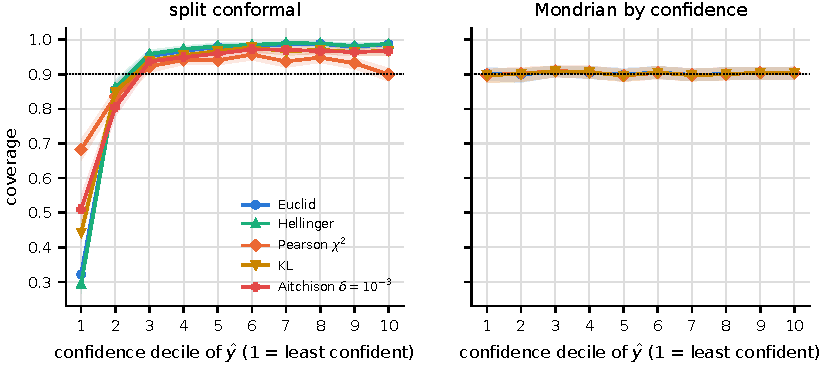
\includegraphics[width=\linewidth]{figs/fig_cifar.pdf}
\caption{CIFAR-10H, ResNet-56: coverage per confidence decile of $\yh$ for split conformal (left) and Mondrian by confidence (right); bands: 95\% bootstrap over images.}\label{fig:cifar}
\end{figure}

\textbf{CIFAR-10H.} All methods are marginally valid (coverage $0.899$--$0.903$, \cref{tab:real}), yet \cref{fig:cifar} shows that every split-conformal score under-covers the least confident decile (coverage $0.29$ Hellinger, $0.32$ Euclid, $0.44$ KL, $0.51$ Aitchison with $\delta=10^{-3}$, $0.68$ $\chi^2$) and over-covers confident images (up to $0.99$). $G_{\rm conf}$ is $0.22$--$0.61$ against a null floor of $0.021$, and it remains $\ge0.13$ for every predictor we tried (raw softmax, ResNet-20, VGG-11; App.\ \cref{tab:cifarfull}). Pearson $\chi^2$---the winner on synthetic Dirichlet data---is the least bad ($G_{\rm conf}=0.22$) and gives the smallest region ($\log M_1=-13.2$), but its coverage drifts \emph{down} again in the most confident decile ($0.90$), so Dirichlet-matched geometry does not transfer: 80\% of target entries are exact zeros, and 44\% of targets are vertices (where all Fisher-type scores coincide with LAC, \cref{prop:lac}).
Conditioning removes only the conditioned variable's gap: Mondrian by confidence reaches $G_{\rm conf}=0.009$ (below the null floor) but \emph{raises} $G_{\rm class}$ (Euclid $0.09\to0.13$, KL $0.09\to0.15$, $\chi^2$ $0.13\to0.15$) and gives much smaller regions on average (log-mass $-14.5$ to $-16.0$ vs.\ $-8.0$ to $-13.2$ unconditioned); Mondrian by predicted class reaches $G_{\rm class}=0.005$ and leaves $G_{\rm conf}$ at $0.2$--$0.5$.
The Aitchison score is \emph{not a single method}: with $\delta=10^{-4},10^{-3},10^{-2},10^{-1}$, $G_{\rm conf}=0.32,0.39,0.47,0.54$ and $\log M_1=-0.12,-1.9,-5.8,-6.6$; a region of log-mass $-0.12$ is essentially the whole simplex. A comparison of Aitchison against other geometries on zero-rich data is therefore a comparison with the choice of $\delta$. A global-covariance ellipsoid in ilr coordinates (fitted on the 1000 held-out images, $\delta=10^{-2}$) behaves like the Aitchison score ($G_{\rm conf}=0.46$ vs.\ $0.47$). The ranking is stable across $\alpha\in\{0.05,0.1,0.2\}$ ($\chi^2$ lowest $G_{\rm conf}$: $0.064,0.217,0.513$), but gaps grow with $\alpha$ (App.\ \cref{tab:alpha}).

\textbf{ChaosNLI} (\cref{tab:real}, right; RoBERTa-large, $T$ fitted on 500 items). With 3 components and 7.9\% zeros the picture differs: for all scores except $\chi^2$ the confidence gap ($0.035$--$0.065$) is close to the null floor of this test-set size ($0.045$); $\chi^2$ is worst ($0.081$, lowest-decile coverage $0.82$) \emph{while} giving the smallest region ($\log M_1=-0.70$ vs.\ $-0.53$ for Hellinger): size alone would pick the geometry with the worst conditional coverage, the situation P3 warns about. With the raw over-confident softmax ($T=1$) the gaps grow to $0.08$--$0.09$ (Euclid, TV, Hellinger, Mahalanobis), $0.15$ (KL), $0.22$ (Aitchison, $\delta=10^{-3}$) and $0.29$ ($\chi^2$, lowest-decile coverage $0.61$) with $\chi^2$ again the smallest region ($-1.03$), the pattern of the synthetic misfit experiment (\cref{sec:misfit}); the distilled model gives a similar picture at $T$ fitted ($\chi^2$ $0.10$, Mahalanobis with $\delta=10^{-3}$ $0.14$, the others $\le0.06$; App.\ \cref{tab:nlifull,tab:nliraw,tab:nlidistil}). The pattern is dataset-specific: on CIFAR-10H the raw softmax leaves $\chi^2$ best ($0.205$ vs.\ $0.23$--$0.46$ for the others). Regions are large in absolute terms because human label distributions on this subset are dispersed (geometric-mean mass $e^{-0.53}=0.59$ of the simplex for Hellinger and $e^{-0.70}=0.50$ for $\chi^2$ at fitted $T$).
